In questo capitolo bla bla bla sezione .... \hl{Aggiungere}

\section{Introduzione}
\label{sec:arte_intro}
\paragraph{Optical Character Recognition}
Ad oggi, sempre più libri cartacei, riviste e giornali presenti in biblioteche e archivi storici stanno venendo trasformati in versioni elettroniche che possono essere manipolate da un computer. A questo scopo, nel corso degli anni sono state sviluppate tecnologie di Optical Character Recognition (comunemente abbreviato con OCR) per tradurre le scansioni e immagini di documenti testuali in testo interpretabile e processabile da un computer. Questi sistemi, però, non sono perfetti e possono introdurre errori nel testo. Può accadere, infatti, che durante il processo di scansione alcuni caratteri vengano letti in modo errato, altri vengano aggiunti e altri ancora non riconosciuti. \E, ad esempio, particolarmente probabile che caratteri o sequenze di caratteri graficamente simili come \textit{"li"} e \textit{"n"} vengano scambiati fra di loro\cite{ocr_error_analysis}. La frequenza di tali errori è influenzata da fattori quali la condizione di deterioramento di un documento e la qualità di acquisizione dell'immagine\cite{hartley1999quality}: la presenza di granelli di polvere, caratteri scoloriti, pagine ingiallite o artefatti risultati dalla scansione, ad esempio, influiscono negativamente sulle performance dei sistemi OCR.\\
La presenza di tali errori in corpora acquisiti tramite OCR risulta problematica in quanto rende meno precisi task di Natural Language Processing (NLP) come, ad esempio, l'esecuzione di query \cite{impatto_ocr_1} o il topic modelling\cite{impatto_ocr_2}. Per ovviare a tali problemi, sono state sviluppate varie soluzioni che mirano a minimizzare il quantitativo di errori presenti nel testo estratto. \E\ possibile classificare queste soluzioni nelle seguenti due categorie:
\begin{itemize}
\item \textbf{OCR Pre-processing}: ricadono in questa categoria tutte quelle tecniche che mirano ad ottenere migliori risultati dall'estrazione del testo attraverso il miglioramento dell'input, ovvero delle immagini, che viene usato dai software di OCR. Tali metodi includono, ma non si limitano a, l'uso di migliori tecniche di scansione, la correzione del contrasto nell'immagine\cite{holley2009good} e la rotazione e correzione di deformazioni nell'immagine\cite{bieniecki2007image} (\autoref{fig:art_prep_ex}).
\begin{figure}[H]
\centering
{
\begin{minipage}{0.35\textwidth}
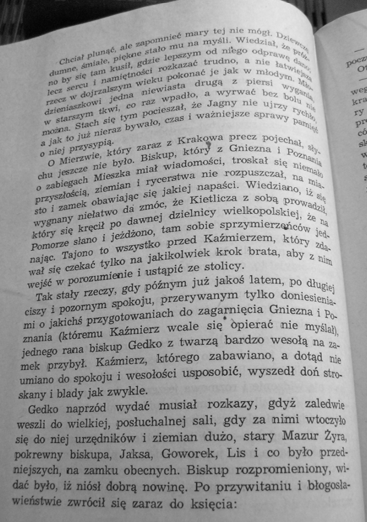
\includegraphics[width=\textwidth]{immagini/stato_arte/prep1}
\end{minipage} 
\begin{minipage}{0.06\textwidth}
\centering
\Large$\rightarrow$
\end{minipage}
\begin{minipage}{0.35\textwidth}
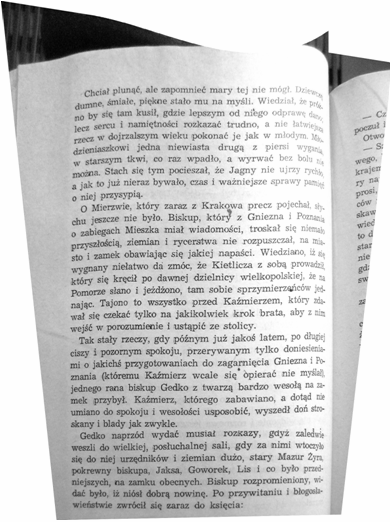
\includegraphics[width=\textwidth]{immagini/stato_arte/prep2}
\end{minipage}
\caption{A sinistra foto di una pagina contenente del testo. A destra, foto della stessa pagina pre-processata per facilitare l'estrazione del testo. Esempio preso da \cite{bieniecki2007image}.}
\label{fig:art_prep_ex}
}
\end{figure}

 
\item \textbf{OCR Post-processing}: ricadono in questa categoria tutte quelle tecniche che mirano ad individuare e correggere gli errori presenti nell'output generato dai vari software di OCR. Essendo l'OCR Post-processing oggetto di questa tesi, sarà approfondito a parte nella \autoref{sec:art_post_post}.
\end{itemize}


OCR pre-processing e post-processing sono spesso usati in congiunzione per ottenere migliori risultati dall'estrazione del testo.

\section{OCR Post-processing}
\label{sec:art_post_post}
In letteratura sono presenti numerosi approcci al problema dell'OCR post-processing, molti dei quali adottano strategie molto differenti. Dato ciò, non è possibile delineare una metodologia generale che ogni approccio segue, ma, in generale, ogni approccio deve:
\begin{enumerate}
\item \textbf{Identificare gli errori} (Error Detection), ovvero delimitare tutte le sezioni contenenti errori nel testo, senza delimitare sezioni corrette. \hl{Espandere?}
\item \textbf{Correggere gli errori} (Error Correction), ovvero ripristinare il testo originale nelle sezioni individuate in precedenza. \hl{Espandere?}
\end{enumerate}

Nelle seguenti sottosezioni sono quindi esposti alcuni dei principali approcci per letteratura, raggruppati nelle seguenti categorie di metodologie:
\begin{itemize}
\item Approcci basati su n-grams
\item Approcci basati su NMT
\item Approcci basati su BERT
\item Altri approcci
\end{itemize}

\hl{Controllo che non sia cambiato niente}

\subsection{Approcci basati su n-grams}
Per discutere gli approcci basati sugli n-grams è prima necessario definire i concetti di token, tokenizzazione e n-gram. 

\paragraph{Token}
\E\ riportata la definizione fornita in \cite{tokendef}: "Un token è una stringa di caratteri contigui compresi fra due spazi, o fra uno spazio e un segno di punteggiatura. Sono token anche [numeri] interi, [numeri] reali o numeri contenenti i due punti (ore, ad esempio 2:00). Tutti gli altri simboli sono considerati essi stessi dei token, eccetto gli apostrofi e i punti di domanda attaccati ad una parola (senza spazi), che in molti casi rappresentano acronimi o citazioni."\\
Più informalmente è possibile associare il concetto di token a quello di parola nel linguaggio naturale.

\paragraph{Tokenizzazione}
Data la precedente definizione di token, per tokenizzazione si intende il dividere un testo, una frase, o più in generale una stringa nei token che la compongono. Data quindi una frase $f \in F$, tokenizzare una frase vuol dire applicare una funzione:
\begin{equation}
\textit{Tok}: F \rightarrow T
\end{equation}
dove ogni $t \in T$ è una lista $[t_1,...,t_n]$ in cui ogni $t_i$ è un token appartenente alla frase iniziale.
Più informalmente quindi, la tokenizzazione restituisce le singole parole appartenenti alla frase iniziale. Ad esempio, data la frase $f_{es}$:
\begin{center}
\textit{"Cantami, o Diva, del pelide Achille
l'ira funesta che infiniti addusse
lutti agli Achei"}
\end{center}
la sua versione tokenizzata $\textit{Tok}(f_{es})$ è:
\begin{center}
[\textit{"Cantami"},
\textit{","},
\textit{"o"},
\textit{"Diva"},
\textit{","},
\textit{"del"},
\textit{"pelide"},
\textit{"Achille"},
\textit{"l'"},
\textit{"ira"},
\textit{"funesta"},
\textit{"che"},
\textit{"infiniti"},
\textit{"addusse"},
\textit{"lutti"},
\textit{"agli"},
\textit{"Achei"}]
\end{center}

\paragraph{n-gram} Un n-gram è una sottosequenza contigua di n elementi di una data sequenza \cite{itwiki:ngram}. Gli elementi in questione possono essere fonemi, sillabe, lettere parole ecc. Nel proseguo di questo documento ogni riferimento a n-gram, salvo indicazione contraria, si riferisce a n-gram di token. Gli n-gram trovano ampio uso nel campo del NLP, dove sono usati, ad esempio, per creare modelli linguistici statistici.\\
In seguito è mostrato un esempio di scomposizione di una frase in n-gram di lunghezza 3, detti quindi 3-gram o trigrams. Dato la frase del precedente esempio $f_{es}$, e data la sua scomposizione in token $\textit{Tok}(f_{es})$, i trigrams formati sono i seguenti:
\begin{center}
\textit{["Cantami", ",", "o"]}, \textit{[",", "o", "Diva"]}, \textit{["o", "Diva", ","]}, \textit{["Diva", ",", "del"]}, \textit{[",", "del", "pelide"]}, \textit{["del", "pelide", "Achille"]}, \textit{["pelide", "Achille", "l'"]}, \textit{["Achille", "l'", "ira"]}, \textit{["l'", "ira", "funesta"]}, \textit{["ira", "funesta", "che"]}, \textit{["funesta", "che", "infiniti"]}, \textit{["che", "infiniti", "addusse"]}, \textit{["infiniti", "addusse", "lutti"]}, \textit{["addusse", "lutti", "agli"]}, \textit{["lutti", "agli", "Achei"]}
\end{center}


\paragraph{Approcci basati su n-grams}
\newcommand{\gw}{GW5}
Gli approcci descritti in questa sezione utilizzano modelli linguistici basati su n-gram per individuare e correggere gli errori. Le soluzioni proposte in questa sezione fanno entrambe uso del Google Web 1T 5-gram dataset\cite{google1t}, che da qui in poi verrà riferito come 	\gw. \gw\ è un dataset contenente n-grams in lingua inglese (da unigrams a 5-grams) associati alla loro frequenza osservata su un totale di 1 trilione di parole. Tutti gli n-grams sono stati estratti attraverso il crawling di pagine web. L'enorme scala del database e la metodologia tramite la quale è stato ottenuto comporta che sia possibile estrarre da \gw\ un amplio lessico che può essere affabilmente usato per fare error detection. Per lo stesso motivo, il dataset si presta bene anche all'applicazione in campi con terminologie di nicchia o altamente specifiche.\\
Il primo approccio trattato quello presentato in \cite{ocrG1}. L'approccio è diviso di tre fasi:
\begin{enumerate}
\item Error Detection: sono usati gli unigram in \gw\ per identificare gli errori. Ogni token all'interno del testo da correggere non presente nella lista degli unigram è considerato un errore. \E\ quindi chiaro come questo metodo riesca ad individuare (e quindi correggere) solo i non-word errors, ovvero tutti quelli errori che risultano in parole non presenti in un dato lessico. Non sono trattati da questo approccio i real-word errors, ovvero tutti quelli errori che risultano in una parola presente in un dato lessico. Si pensi ad esempio alla parola \textit{"sale"} interpretata come \textit{"sala"} da un software OCR.

\item Candidate Spelling Generation: per ogni errore si produce una lista di parole candidate per la correzione. Per fare ciò si scompone la parola errata in 2-grams a livello di carattere. Ad esempio, la parola "sangle" è scomposta in "sa", "an", "ng", "gl", "le". Per ognuna delle parole nel lessico di unigram, in seguito, si conta quante occorrenze dei 2-gram della parola da correggere sono contenute. Ad esempio, la parola "single" contiene tre occorrenze ("ng","gl","le"). Le prime 10 parole con più occorrenze dei 2-gram sono considerate i candidati per la correzione.

\item Error Correction: si considera il 5-gram terminante con la parola errata $[t_1,t_2,t_3,t_4,\textit{err}]$. Per ognuno dei candidati $c_i$ è prodotto il 5-gram $[t_1,t_2,t_3,t_4,{c_i}]$: di questi 5-gram prodotti, quello con più occorrenze all'interno di \gw\ contiene la correzione da applicare.
\end{enumerate}

Un approccio simile è esposto in \cite{ocrG2}. A differenza dell'approccio precedente, l'error detection e la generazione dei candidati non usano \gw, ma sono usate altre tecniche che mirano a correggere anche i real-word errors. L'approccio utilizzato per l'error correction invece sfrutta lo stesso principio di \cite{ocrG1}, ma con una logica leggermente più complessa. Il funzionamento è il seguente:
\begin{enumerate}
\item Error Detection e Candidate Generation: per i non-word errors GNU-Aspell\cite{atkinsongnu} è utilizzato per individuare gli errori e proporre i possibili candidati per la correzione. Per i real-word errors invece, sono usati dei confusion-set pre-definiti per individuare i possibili errori e generare i candidati. Un confusion-set non  è altro che un insieme di parole simili che possono essere confuse fra di loro, come \{they'
re, their, there\}. I candidati per un possibile errore sono quindi le parole appartenenti al suo confusion set.

\item Error Correction. Per ogni candidato si considera un intorno di 2 parole, andando così a comporre un 5-gram. Se il 5-gram in cui è presente l'errore nel testo è $[t_1,t_2,\textit{err},t_3,t_4]$, allora per il candidato $c_i$ sarà $[t_1,t_2,c_i,t_3,t_4]$. Il candidato scelto è quello il cui 5-gram compare più volte in \gw. In caso nessun 5-gram compaia nel dataset, il processo si ripete con il 3-gram $[t_2,c_i,t_3]$ e successivamente solo con l'unigram $[c_i]$, ovvero viene scelto il candidato con la maggior frequenza nel corpus.
\end{enumerate}
Gli approcci descritti fino ad ora, seppur molto efficaci contro i non-word errors, ma non correggono o sono poco efficaci contro i real-word errors e altri tipi di errori. Si pensi ad esempio a situazioni in cui token viene separato da spazi, o in cui due token sono fusi insieme. Inoltre questi approcci, richiedono un'elevata quantità di dati per funzionare efficacemente (\gw\ occupa 87GiB su disco) , il che non li rende facilmente applicabili.

% Potrei aggiungere cose anche da https://aclanthology.org/H05-1109.pdf
% o da https://ieeexplore.ieee.org/stamp/stamp.jsp?tp=&arnumber=8978061

\subsection{Approcci basati su NMT}
%Neural machine translation is a recently proposed approach to machine translation. Unlike the traditional statistical machine translation, the neural machine
%translation aims at building a single neural network that can be jointly tuned to
%maximize the translation performance.
\paragraph{Neural Machine Translation} Il Neural Machine Translation (NMT) è un approccio al machine translation che consiste nella costruzione di un solo neural network che può essere messo a punto singolarmente per massimizzare le performance di traduzione\cite{nmtdef}. I modelli più recenti nel campo del NMT sfruttano la cosiddetta architettura encoder-decoder (\autoref{fig:art_encdec}). Tali modelli sono anche comunemente riferiti come modelli sequence-to-sequence (seq2seq), in quanto trasformano una sequenza di caratteri o lettere appartenente a un dominio (ad esempio quello dell frasi in lingua italiana) ad una sequenza appartenente ad un altro dominio (ad esempio quello delle frasi in lingua inglese). In questi modelli, la frase iniziale passa attraverso l'encoder, che ne restituisce una rappresentazione sotto forma di una lista di valori numerici. Successivamente, questi valori sono dati in input al decoder, che produce una frase con lo stesso significato, ma con il vocabolario e la grammatica della lingua target. Encoder e decoder possono essere implementati con diverse architetture, ma, data la natura dei dati trattati (dati sequenziali, come frasi), sono spesso implementati con dei Recurrent Neural Network (RNN).


\begin{figure}[H]
\centering
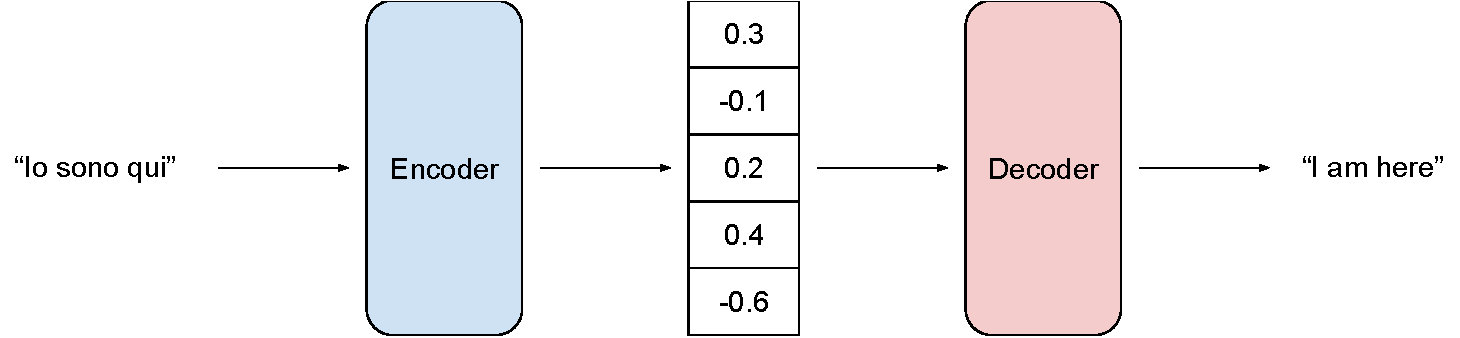
\includegraphics[width=\textwidth]{immagini/stato_arte/encoder_decoder}
\caption{Schema semplificato di un'architettura encoder-decoder che traduce da italiano a inglese}
\label{fig:art_encdec}
\end{figure}

L'idea che gli approcci in questa sezione propongono è quindi quella di trattare il problema della correzione degli errori come un problema di traduzione di sequenze: dato il dominio $E$ delle sequenze contenenti errori, e il dominio $C$ delle sequenze corrette (detto anche Ground Truth, abbreviato GT), il modello seq2seq che effettua la traduzione può essere visto come la seguente funzione:
\begin{equation}
M: E \rightarrow C
\end{equation}
Allo stesso modo, ogni modello necessita prima di essere allenato con corpus parallelo dove ad ogni sequenza $e \in E$ corrisponde un sequenza corretta $c \in C$.

\paragraph{Modelli Word Based e Character based} Come si è visto, i modelli seq2seq trasformano una sequenza in un'altra sequenza. In base al tipo di elementi che compongono tali sequenze, è possibile descrivere due tipologie di modelli:
\begin{itemize}
\item Modelli Word Based (da qui in poi riferiti come WB): in questo tipo modelli un elemento corrisponde ad una parola, o meglio, ad un token. Questo tipo di approcci richiede quindi che tutte le sequenze in $E$ e in $C$ siano tokenizzate. Inoltre, prima dell'allenamento, è necessario estrarre i dizionari della lingua d'origine e della lingua target dai corpora utilizzati.
\item Modelli Character Based (da qui in poi riferiti come CB): in questo tipo di modelli un elemento corrisponde ad un carattere. Prima del training, è necessario estrarre il set di caratteri della lingua d'origine e della lingua target dai corpora utilizzati.
\end{itemize}
Da un'analisi della letteratura, si evince come i modelli CB siano generalmente preferiti per il task dell'OCR Post-Processing\cite{mokhtar2018ocr,hamalainen2019paft,nguyen2020neural,
nastase2018correction,duong2020unsupervised,amrhein2018supervised}.
In \cite{mokhtar2018ocr} viene proposto un confronto sullo stesso corpus fra due architetture molto simili, la prima WB e la seconda CB. Nello studio, gli autori concludono come l'architettura character based produca risultati significativamente migliori. I modelli CB infatti riescono a correggere gli errori a livello di carattere, e ciò comporta i seguenti vantaggi:
\begin{itemize}
\item A differenza dei modelli WB, i modelli CB possono correggere anche errori in parole non presenti nel dizionario estratto.
\item Rispetto ai modelli WB, sono richiesti meno dati durante la fase di allenamento.
\end{itemize}


\paragraph{Approcci basati su NMT}
Il primo approccio presentato è quello descritto in \cite{nguyen2020neural}. Nella soluzione presentata gli autori utilizzano il tool OpenNMT\cite{klein2017opennmt} per allenare un modello CB. Il modello è allenato sia con coppie di sequenze identiche (quindi senza errori) che con sequenze dove la frase acquisita tramite OCR e la GT differiscono. Per queste ultime è adottata la seguente strategia di data augmentation: per ogni errore, si costruiscono cinque 5-gram con il token errato e i suoi token vicini facendo scorrere una finestra sopra la sezione di testo contenente il token errato. In questo modo si producono 5 sequenze diverse che possono essere usate per il training, evitando di un avere un modello con troppo bias verso le sequenze senza errori. L'approccio per la correzione si divide dunque in due fasi: un prima fase di error detection utilizza un modello BERT (si rimanda il lettore alla \autoref{sec:art_bert}) messo a punto per la classificazione per individuare gli errori nelle sequenze; una seconda fase di error correction invece utilizza il modello di NMT allenato precedentemente per correggere gli errori.\\
In \cite{amrhein2018supervised} si utilizza una metodologia simile per il training del modello, sviluppato con il framework Nematus\cite{sennrich2017nematus}. Questo approccio utilizza una tecnica chiamata "factored NMT", utilizzata anche in \cite{nguyen2020neural}, che permette di aggiungere informazioni strutturate alle sequenze in input. Ad esempio, è possibile aggiungere ad ogni carattere della sequenza informazioni sull'identificativo e l'anno del corpus di provenienza. Ciò permette di usare più corpora eterogenei per l'allenamento di un solo modello, aumentando così i dati a disposizione.\\
\cite{nastase2018correction} propone invece un approccio per correggere unicamente i word segmentation errors (si rimanda il lettore alla \autoref{sec:met_introduzione}), ovvero errori introdotti da spazi spuri che influiscono sulla segmentazione del testo. La metodologia proposta allena un modello su coppie di sequenze così composte: la sequenza target è una sequenza corretta senza errori; la sequenza di input invece è la sequenza target senza spaziature. In questo modo, il modello è allenato per inserire correttamente gli spazi e può essere usato per correggere i word segmentation error.\\
In \cite{hamalainen2019paft} si propone invece un approccio per il post processing e l'allenamento di un modello di NMT senza disporre di un corpus parallelo. L'approccio propone di allenare modello Word2Vec direttamente sul corpus contenente gli errori introdotti dal software di OCR. Dopodiché, per ogni parola estratta corretta (la correttezza è verificata attraverso un dizionario) si usa il modello Word2Vec per trovare le parole semanticamente più simili. Di queste, quelle con distanza di Levenshtein minore o uguale di 3 sono considerate versioni errate della parola corretta. Successivamente, le coppie di parole corrette e parole versione errate sono usate per allenare il modello di NMT, che è poi utilizzato per la correzione. Dato che il risultante modello è allenato per la correzione di singole parole, gli errori di segmentazione non vengono corretti. Inoltre, si rende necessaria una fase di error detection basata su un dizionario. \\
L'approccio proposto è ulteriormente sviluppato in \cite{duong2020unsupervised}. Gli autori procedono sempre con la creazione di un corpus parallelo per l'allenamento di un modello di NMT, ma con una diversa strategia. In questo caso si parte da sequenze senza errori, che fungono da input per l'allenamento, e si creano sequenze target mediante l'introduzione di errori in maniera controllata. Inoltre, in questo caso, le sequenze usate per l'allenamento sono degli 5-gram centrati sulla parola errata, con lo scopo di fornire un maggior contesto per migliorare la correzione.


\subsection{Approcci basati su BERT}
\label{sec:art_bert}

% Non devo per forza citare 50 mila paper
% Dico che c'è la possibilità che il soft masking possa funzionare e porto le prove



\subsection{Altri Approcci}
























